% Authors: Sukrit Arora, Rohan Suresh, Henry Sun
% Emails: sukrit.arora@berkeley.edu, 
Consider the basic problem of finding some $\vec{x}$ such that $\mathbf{A}\vec{x} = \vec{b}$. If we have an equal number of equations as unknowns, then we are pretty happy.\\

In many cases, however, we cannot find a solution, as the set of equations that are described by $\mathbf{A}$ and $\vec{b}$ are overdetermined (i.e. there are more equations than there are unknowns).\\

In general, least squares involves finding the best approximate solution to these overdetermined systems.\\
    
Looking at this graphically, we can think of the problem of data-fitting. That is to say that we have many samples, and we want to draw a straight line that goes as close to each point as possible.\\

\begin{enumerate}

\item{Looking at the plot below, setup a system of linear equations describing a line going through each point.\\

\begin{center}
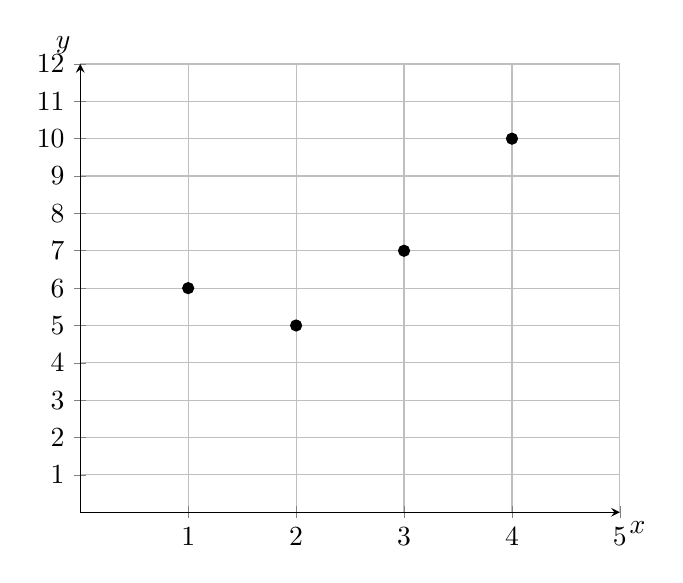
\begin{tikzpicture}[>=latex]
\begin{axis}[
  axis x line=center,
  axis y line=center,
   xtick={0,...,5},
  ytick={0,...,12},
  xlabel={$x$},
  ylabel={$y$},
  xlabel style={below right},
  ylabel style={above left},
  xmin=0,
  xmax=5,
  ymin=0,
  ymax=12,
  grid]
  \addplot [only marks] table {
    1 6
    2 5
    3 7   
    4 10
 };
\end{axis}
\end{tikzpicture}
\end{center}
}
    
\sol{
    Recall that the generalized equation for a line is $y=mx+c$, where $m$ is the slope of the line and $c$ is a constant shift. Since we have 4 points, we have 4 equations with known ($x$,$y$) values, and unknown slope and constants ($m$ and $c$).
    
    $$6 = (1)m + c$$
    $$5 = (2)m + c$$
    $$7 = (3)m + c$$
    $$10 = (4)m + c$$
    
}

\item{
    Put this system of linear equations into matrix-vector form.
}

\note{
  If students are confused about how to populate A, expand out the multiplication Ax and show that doing so recovers the original system of equations.
}

\sol{



    $\mathbf{A}$: A matrix whose rows contain coefficients for our $x_i$.
    \[\mathbf{A} = \begin{bmatrix}1&1\\2&1\\3&1\\4&1\end{bmatrix}\]
    $\vec{x}$: A vector containing the parameters that we want to be optimizing
    \[\vec{x} = \begin{bmatrix}m\\c\end{bmatrix}\]
    $\vec{b}$: A vector containing the "true" y values of our original points, which we will want our $\hat{x}$ to approximate
    \[\vec{b} = \begin{bmatrix}6\\5\\7\\10\end{bmatrix}\]

    Putting this into the standard form $\mathbf{A}\vec{x}=\vec{b}$, we get:
    
    $$\begin{bmatrix}1&1\\2&1\\3&1\\4&1\end{bmatrix}\begin{bmatrix}m\\c\end{bmatrix} = \begin{bmatrix}6\\5\\7\\10\end{bmatrix}$$
    
    }
    
\item{
    Given that $(\mathbf{A}^T\mathbf{A})^{-1} = \begin{bmatrix}0.2&-0.5\\-0.5&1.5\end{bmatrix}$, use the linear least squares technique you learned earlier on this overdetermined system to solve for a line of best fit
}

\sol{
    $$\hat{x} = (\mathbf{A}^T\mathbf{A})^{-1}\mathbf{A}^T\vec{b}$$
    $$= \begin{bmatrix}0.2&-0.5\\-0.5&1.5\end{bmatrix}\begin{bmatrix}1&2&3&4\\1&1&1&1\end{bmatrix}\begin{bmatrix}6\\5\\7\\10\end{bmatrix}$$
    $$= \begin{bmatrix}0.2&-0.5\\-0.5&1.5\end{bmatrix}\begin{bmatrix}77 \\ 28 \end{bmatrix}$$
    $$\hat{x} = \begin{bmatrix}1.4 \\ 3.5 \end{bmatrix}$$
    
    Thus, we see that the line of best fit has a slope of $1.4$ and a constant shift of $3.5$, and the equation of the line is $y = 1.4x + 3.5$
}

\item{
   Plot this line in the plot above.
}

\sol{
    \begin{center}
    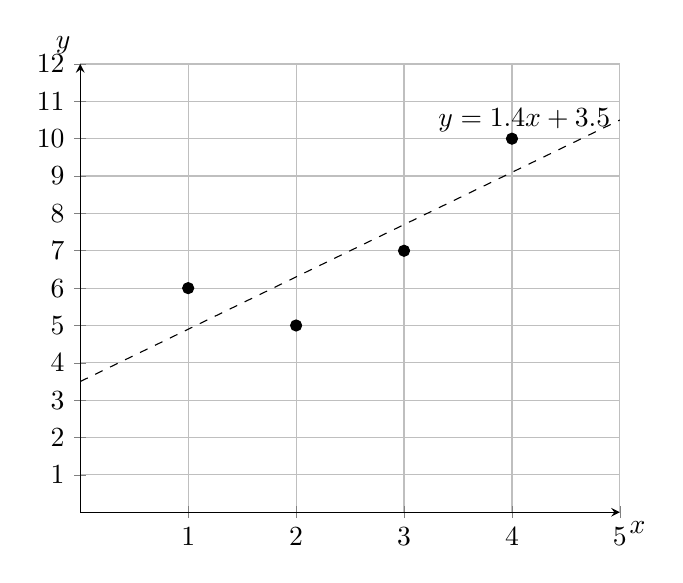
\begin{tikzpicture}[>=latex]
    \begin{axis}[
      axis x line=center,
      axis y line=center,
       xtick={0,...,5},
      ytick={0,...,12},
      xlabel={$x$},
      ylabel={$y$},
      xlabel style={below right},
      ylabel style={above left},
      xmin=0,
      xmax=5,
      ymin=0,
      ymax=12,
      grid]
     \addplot [only marks] coordinates {
        (1,6)
        (2,5)
        (3,7)  
        (4,10)
    };
     
     \addplot [domain=0:5, samples=2, dashed] {1.4*x+3.5} node[left,pos=1] {$y = 1.4x+3.5$}; ;
     
    \end{axis}
    \end{tikzpicture}
    \end{center}
}
    
\item{
C.F. Gauss (the 19th century mathematician of Gaussian elimination fame) used least squares to model the orbits of various celestial bodies around the sun. From Kepler’s laws of planetary motion, Gauss constructed the following equation:
$$\alpha x^2 + \beta xy + \gamma y^2 + \delta x + \epsilon y = 1$$ where x and y describe the position of the object in the 2D plane of its orbit around the sun, and the Greek letters are unknown coefficients.
A scientist named Piazzi observed the orbit of the dwarf planet Ceres over the period of a month, producing 19 data points of its xy-coordinates. Given this data, how might Gauss have used least squares to recover appropriate values of the coefficients alpha, beta, gamma, delta, epsilon to model the orbit of Ceres?}

\note{
  This subpart is interesting because it uses least squares to solve a system of equations that we might at first glance consider nonlinear. Emphasize to students that x and y in this problem are data points, and our variables of interest are coefficients; the equations are still linear in our coefficients.
}

\sol{
The question we need to ask is: what are the variables we need to solve for? In this case, we have points in space: thus, we have values of $x$ and $y$. Using these two values, we can also easily find $x^2$, $xy$, and $y^2$. So, the unknowns in this story are the coefficients of these variables, or the "weights" of each term. Thus we can set this problem for $n$ measurements in the form of $\mathbf{A}\vec{x}=\vec{b}$:
$$\begin{bmatrix}x_1^2&x_1y_1&y_1^2&x_1&y_1\\x_2^2&x_2y_2&y_2^2&x_2&y_2\\ & & \vdots \\x_n^2&x_ny_n&y_n^2&x_n&y_n\end{bmatrix}\begin{bmatrix}\alpha \\ \beta \\ \gamma \\ \delta \\ \epsilon \end{bmatrix} = \begin{bmatrix}1 \\ 1 \\ \vdots \\ 1 \end{bmatrix}$$

In this case, we have an overdetermined system, which  (as we've explored earlier) can be solved using least squares. Simply use the least squares formula to find the best approximation to your weights $\hat{x} = (\mathbf{A}^T\mathbf{A})^{-1}\mathbf{A}^T\vec{b}$

Then, you can plot an ellipse of best fit that models the path of the planetary body.

\begin{figure}[H]
  \begin{center}
    \includegraphics[width=5cm,height=5cm,keepaspectratio]{../planet_path.jpg}
  \end{center}
\end{figure}
}


    
\end{enumerate}